
%% A sample appendix
%%
%%**********************************************************************
%% Legal Notice:
%% This code is offered as-is without any warranty either
%% expressed or implied; without even the implied warranty of
%% MERCHANTABILITY or FITNESS FOR A PARTICULAR PURPOSE!
%% User assumes all risk.
%% In no event shall any contributor to this code be liable for any damages
%% or losses, including, but not limited to, incidental, consequential, or
%% any other damages, resulting from the use or misuse of any information
%% contained here.
%%**********************************************************************
%%
%% $Id: Appendix.tex,v 1.5 2006/08/24 21:12:47 Owner Exp $
%%

% N.B.: an appendix chapter starts with "appchapter" instead of "chapter"
%
% The first argument in [ ] is the title as displayed in the table of contents
% The second argument is the title as displayed here.  Use \\ as appropriate in
%   this title to get desired line breaks
\appchapter[NVM Middlewre Concurrency Control Results]{NVM Middlewre Concurrency Control Results}
\label{appendix:b}

% \begin{figure}[ht]
%     \centering
%     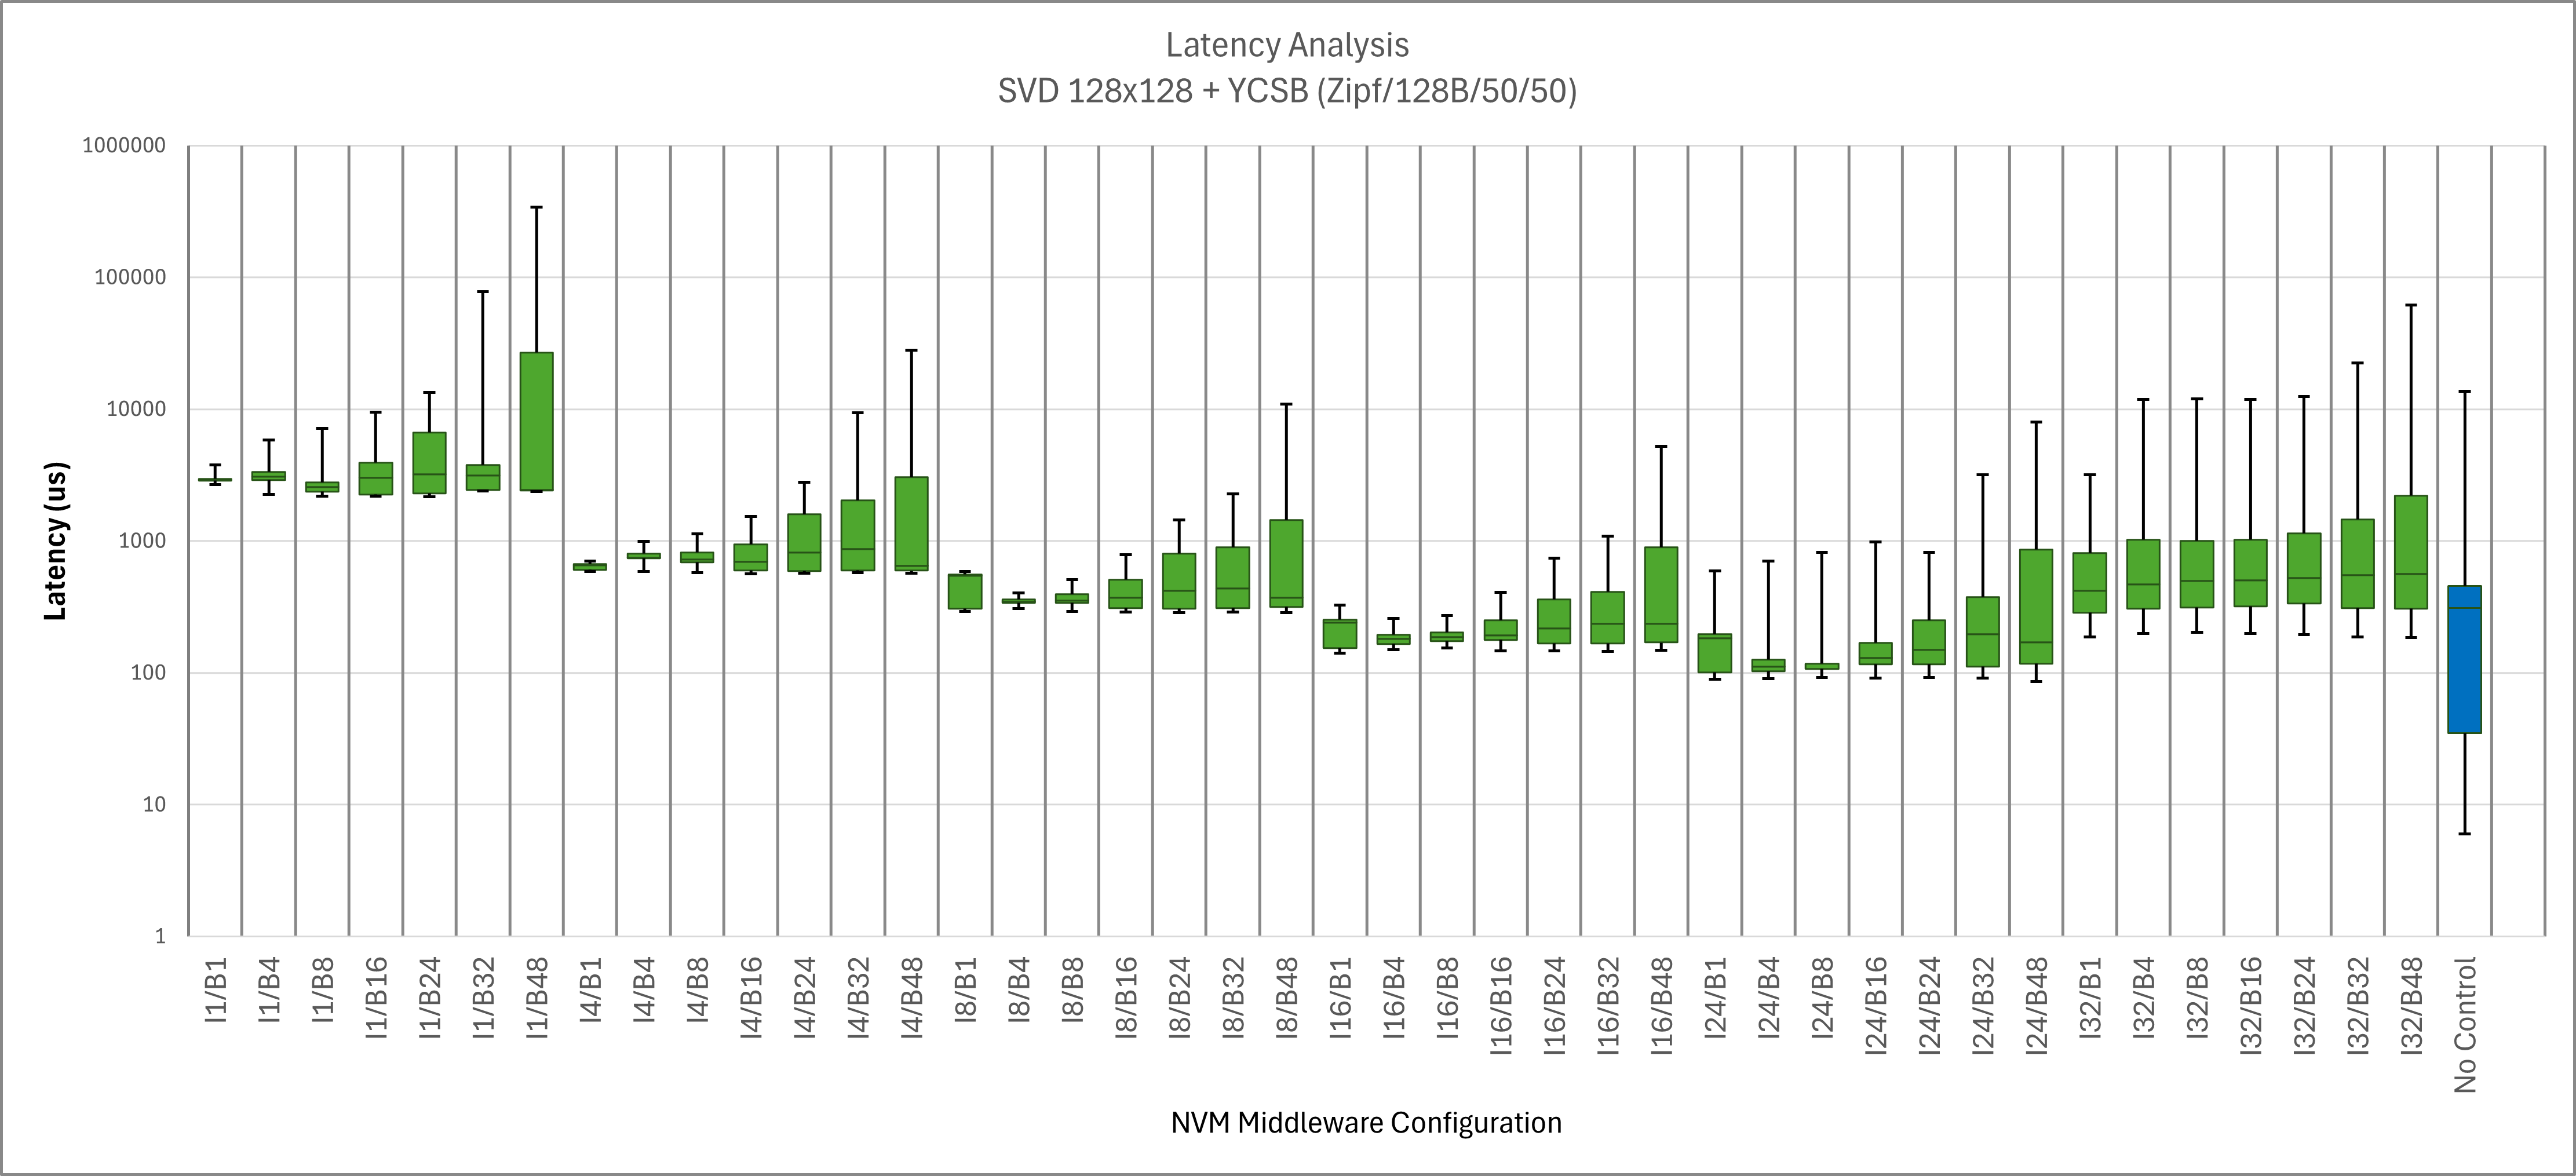
\includegraphics[width=\textwidth,height=\textheight,keepaspectratio,angle=0]{images/middleware-latency.png}
%     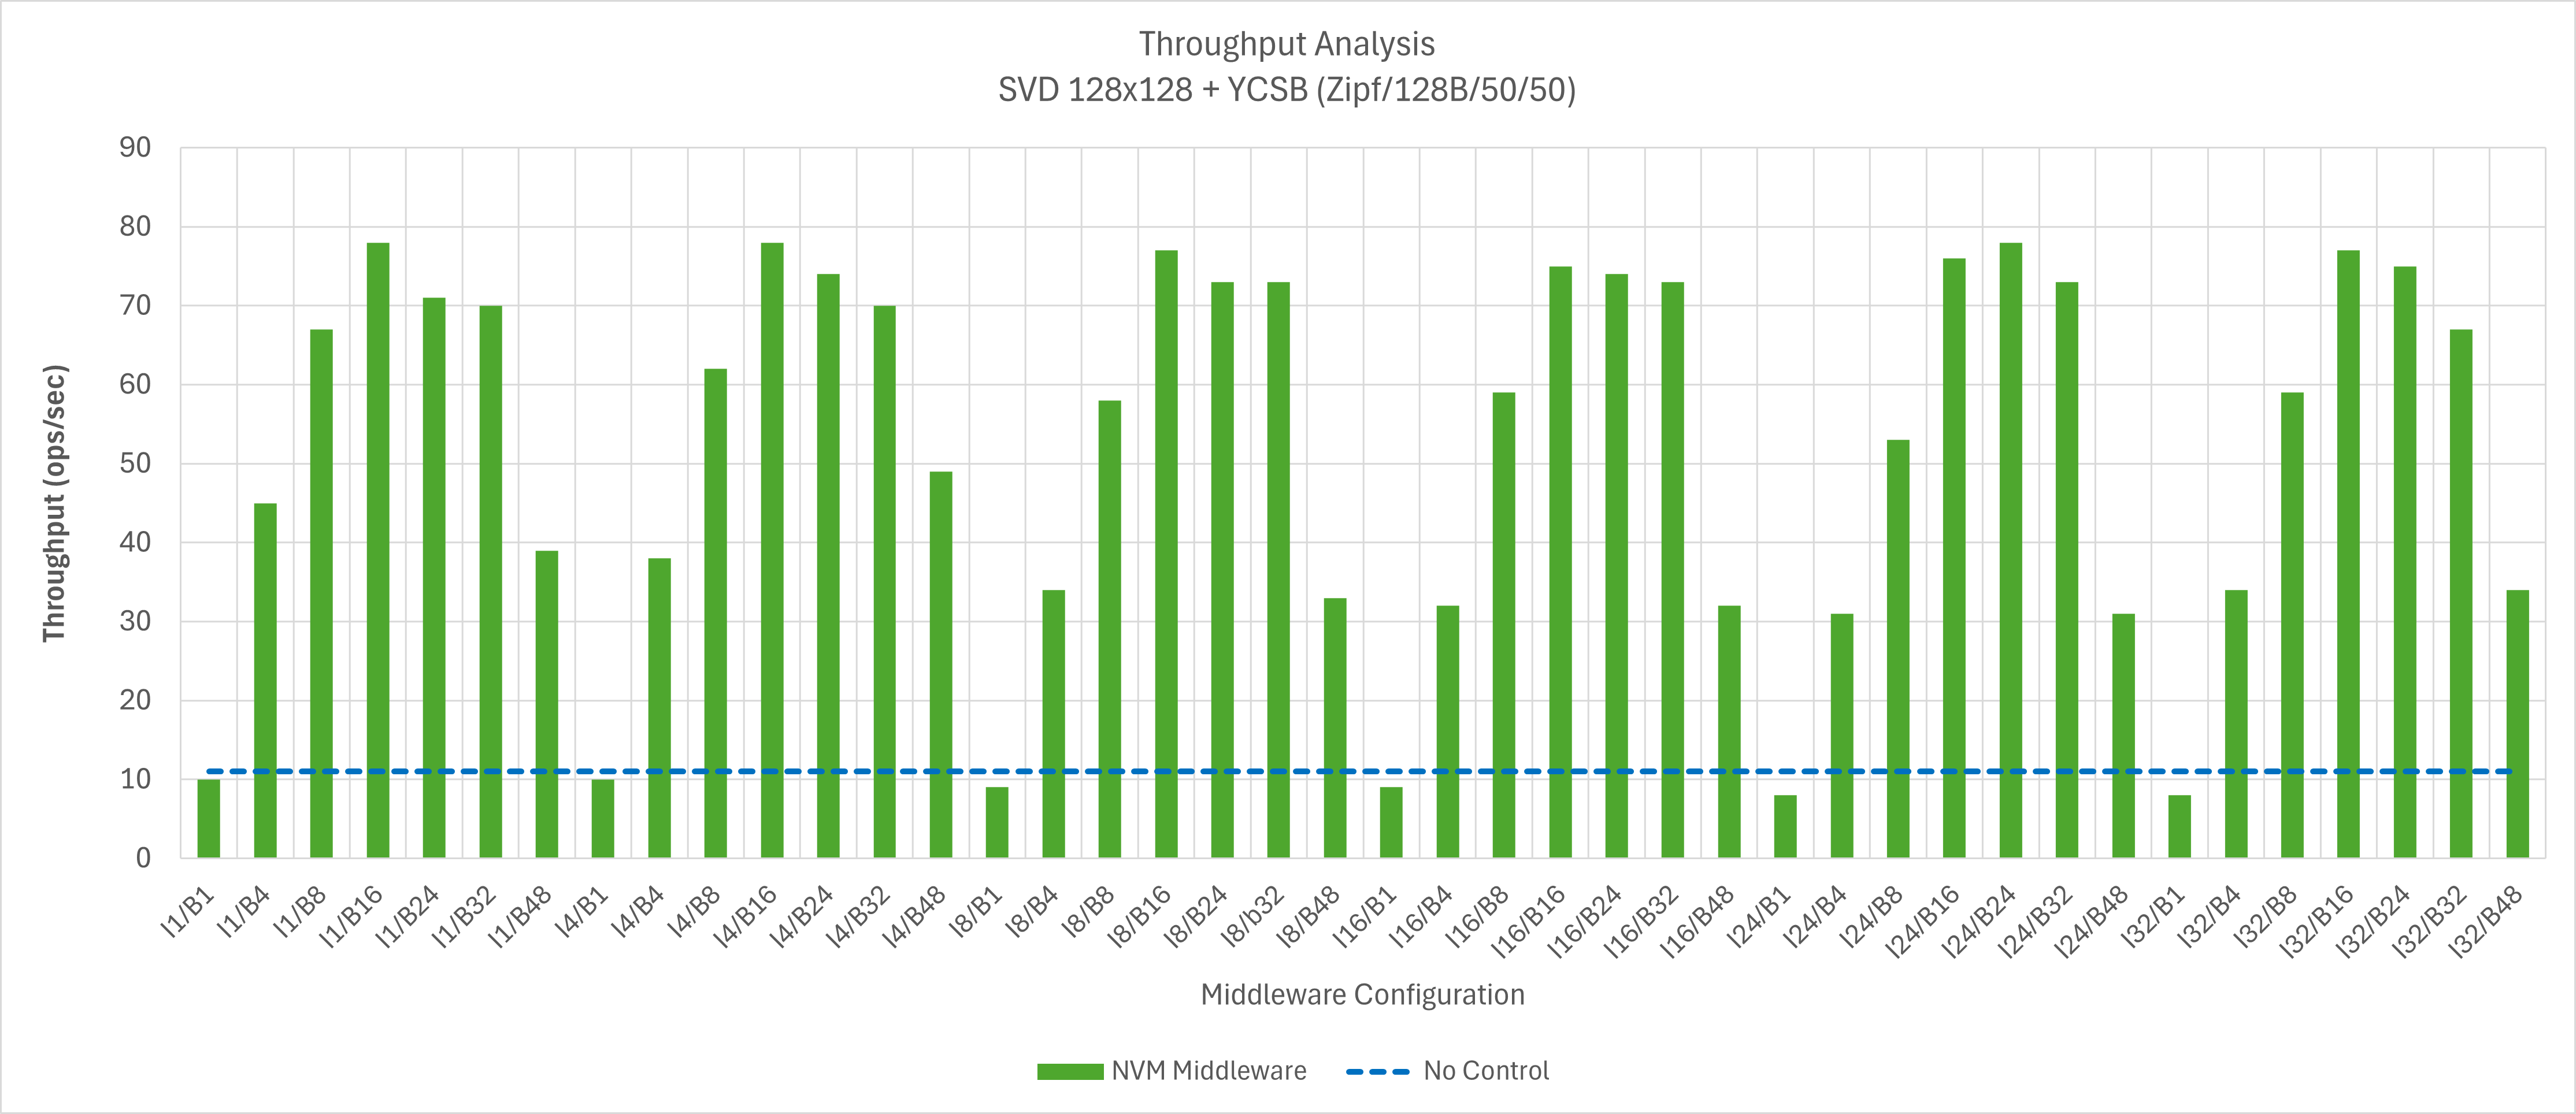
\includegraphics[width=\textwidth,height=\textheight,keepaspectratio,angle=0]{images/middleware-tp.png}
%     \caption{Middleware Evaluation}
%     \label{fig:middleware_eval}
%   \end{figure}

\begin{figure}[ht]
  \centering
  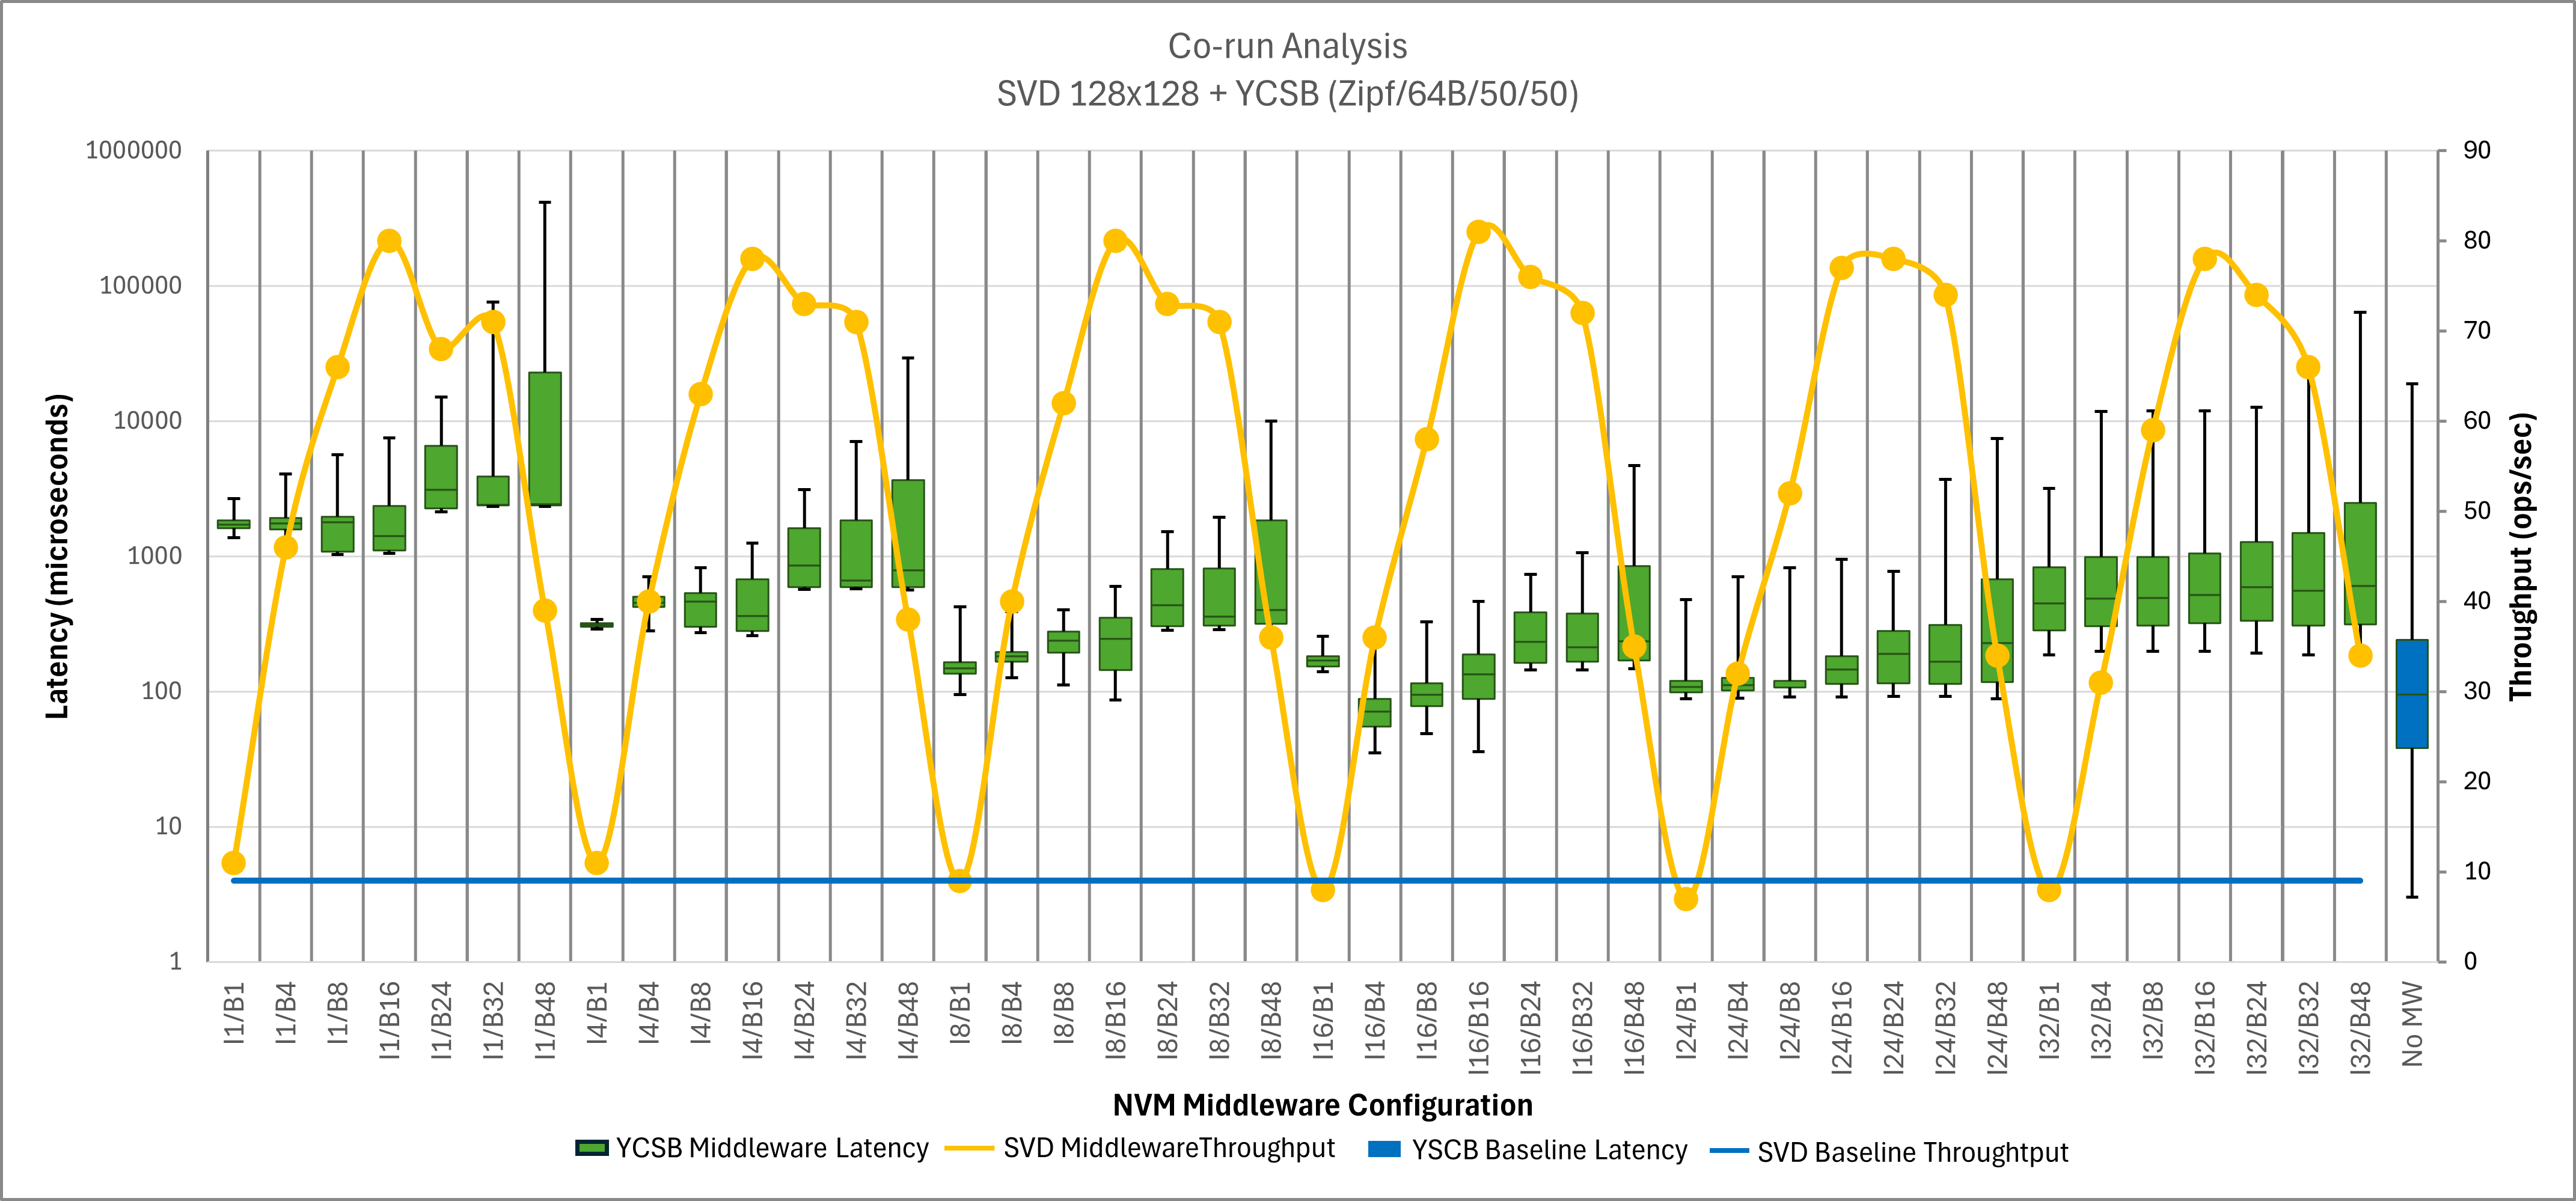
\includegraphics[width=0.8\textwidth,height=\textheight,keepaspectratio,angle=0]{images/64b_50_50_middleware_eval.png}
  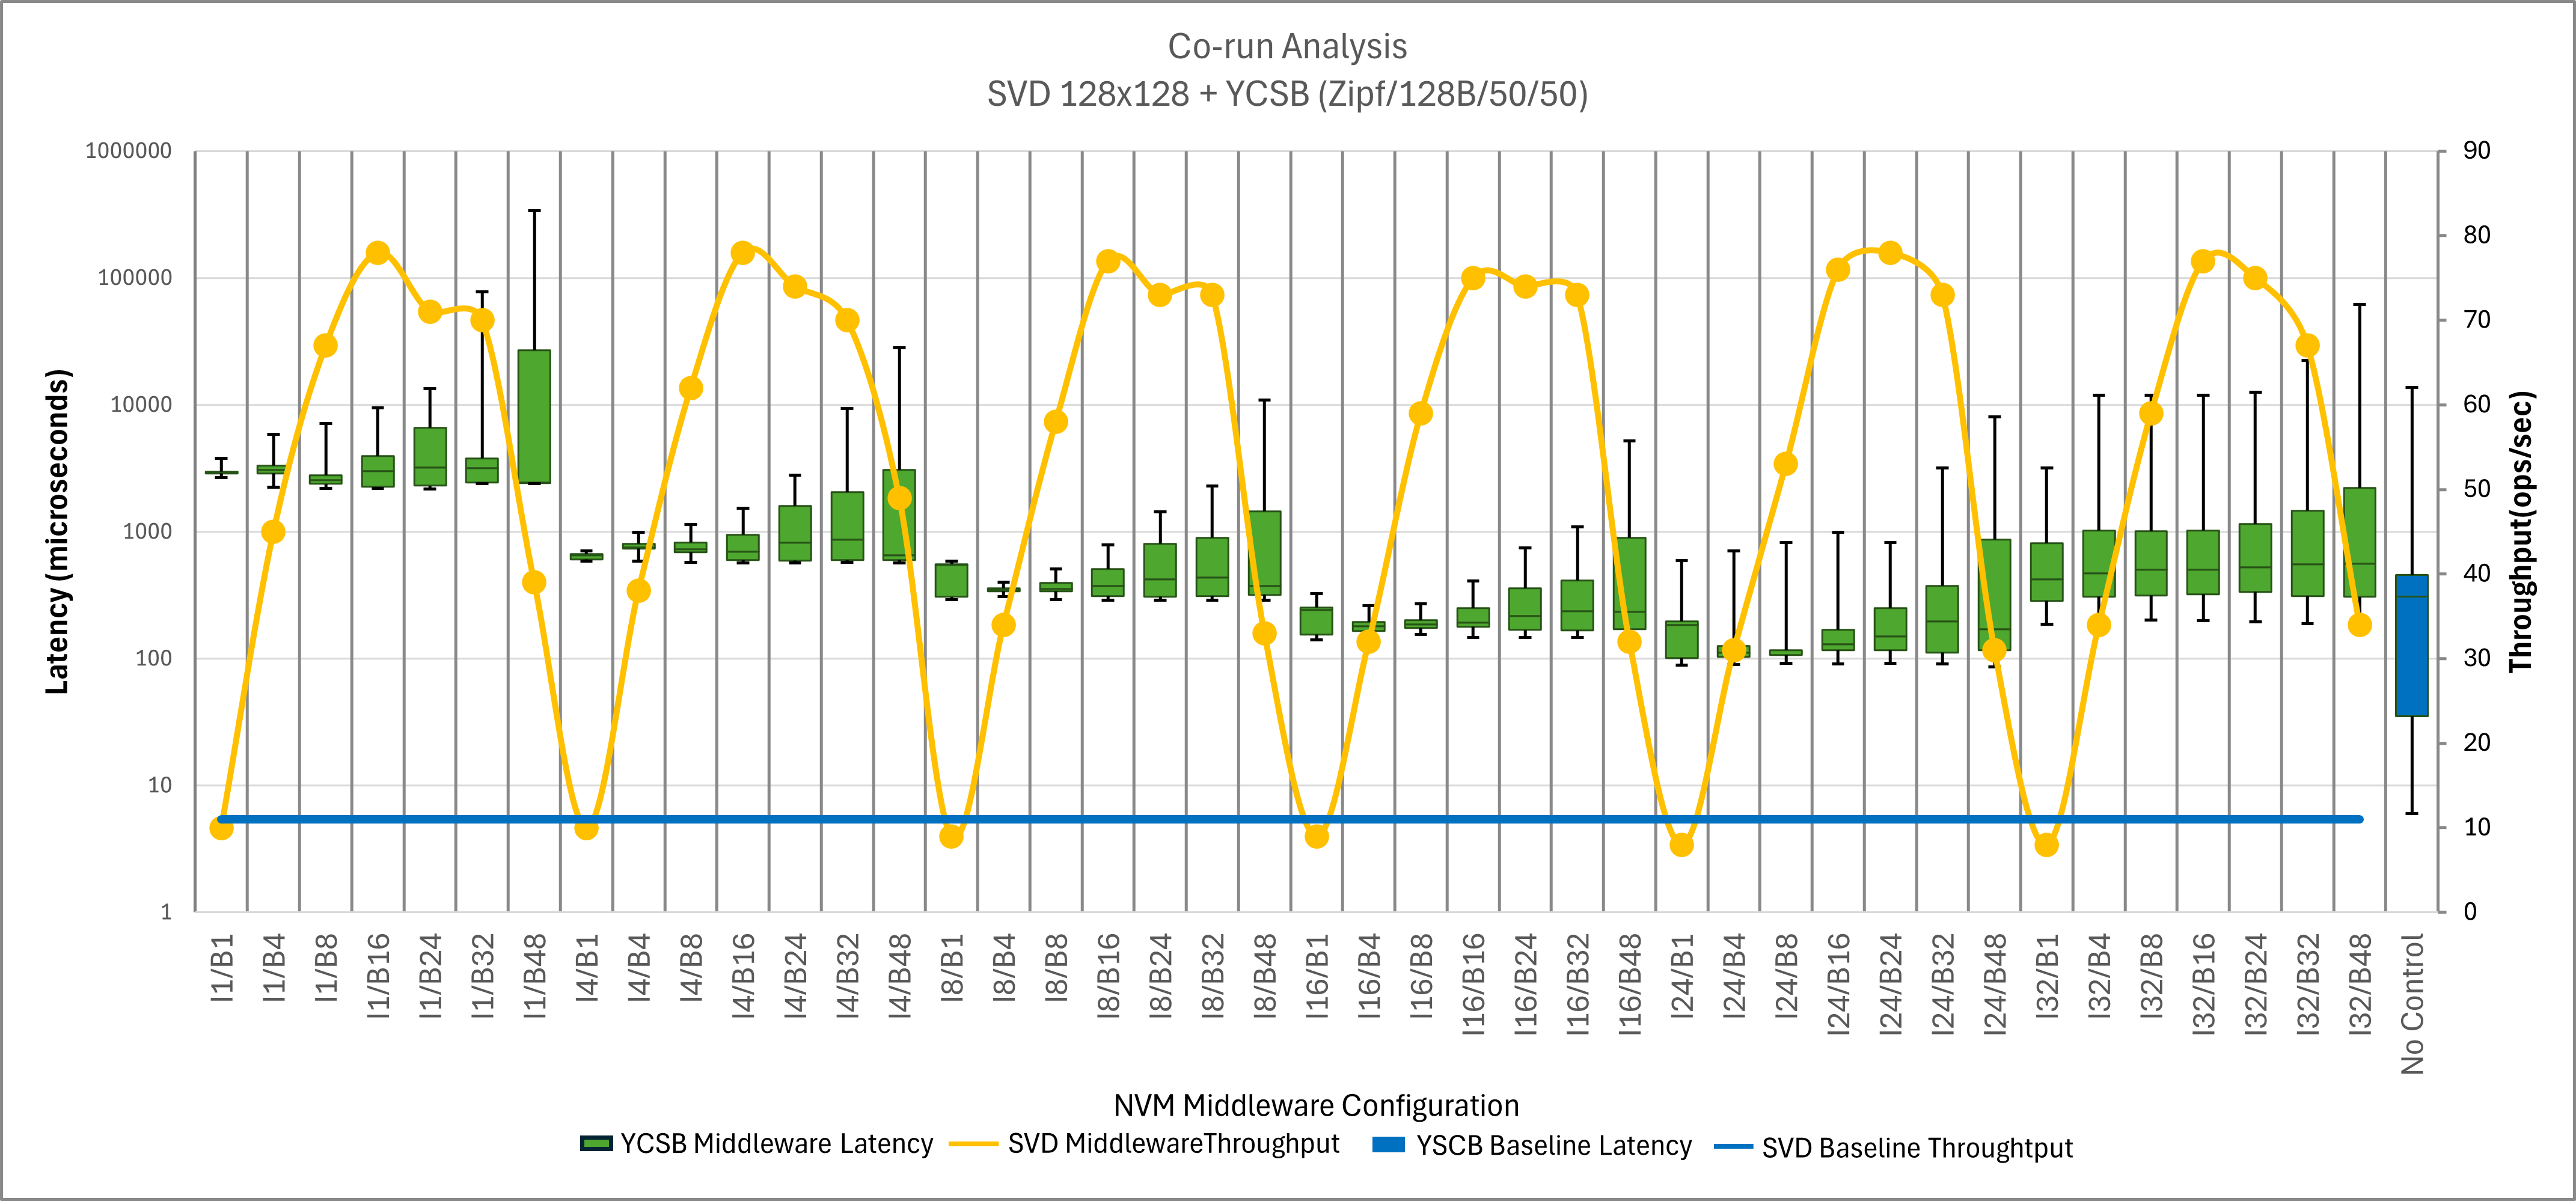
\includegraphics[width=0.8\textwidth,height=\textheight,keepaspectratio,angle=0]{images/128b_50_50_middleware_eval.png}
  % \caption[Evaluation of NVM Middleware: Benchmark A]{Evaluation of the NVM Middleware's concurrency control mechanism when co-running a batch workload and a interactive workload with Zipfian request distribution and even distribution of read and write requests. The interactive workload is generated by YCSB, and two runs are performed configuring YCSB with 64B and 128B data access sizes. Both applications utilize 100 client threads to send requests to the NVM Middleware. The throughput (yellow line) and 99th percentile latency (green box plot) of each application are observed and compared against a baseline with no concurrency control (blue line and box plot).}
  \caption[Evaluation of NVM Middleware: Benchmark A]{Evaluation of the NVM Middleware's concurrency control mechanism when co-running SVD I/O traces (batch) and a YCSB workload (interactive) configured with zipfian request distribution and an even distribution of read and write requests. Two runs are performed configuring YCSB with 64B and 128B data access sizes. Both applications utilize 100 client threads to send requests to the NVM Middleware. The illustration presents statistics on throughput (yellow line) and 99th percentile latency (green box plot) obtained under different configurations of the NVM Middleware, denoted as $I/B$ (Interactive threads/Batch threads). These statistics are compared against a baseline scenario with no concurrency control (blue line and blue box plot). The latencies observed by YCSB are depicted as a distribution, ranging from the minimum to the maximum observed, along with quartiles and median values.}
  \label{fig:50_50_middleware_eval}
\end{figure}

\begin{figure}[ht]
  \centering
  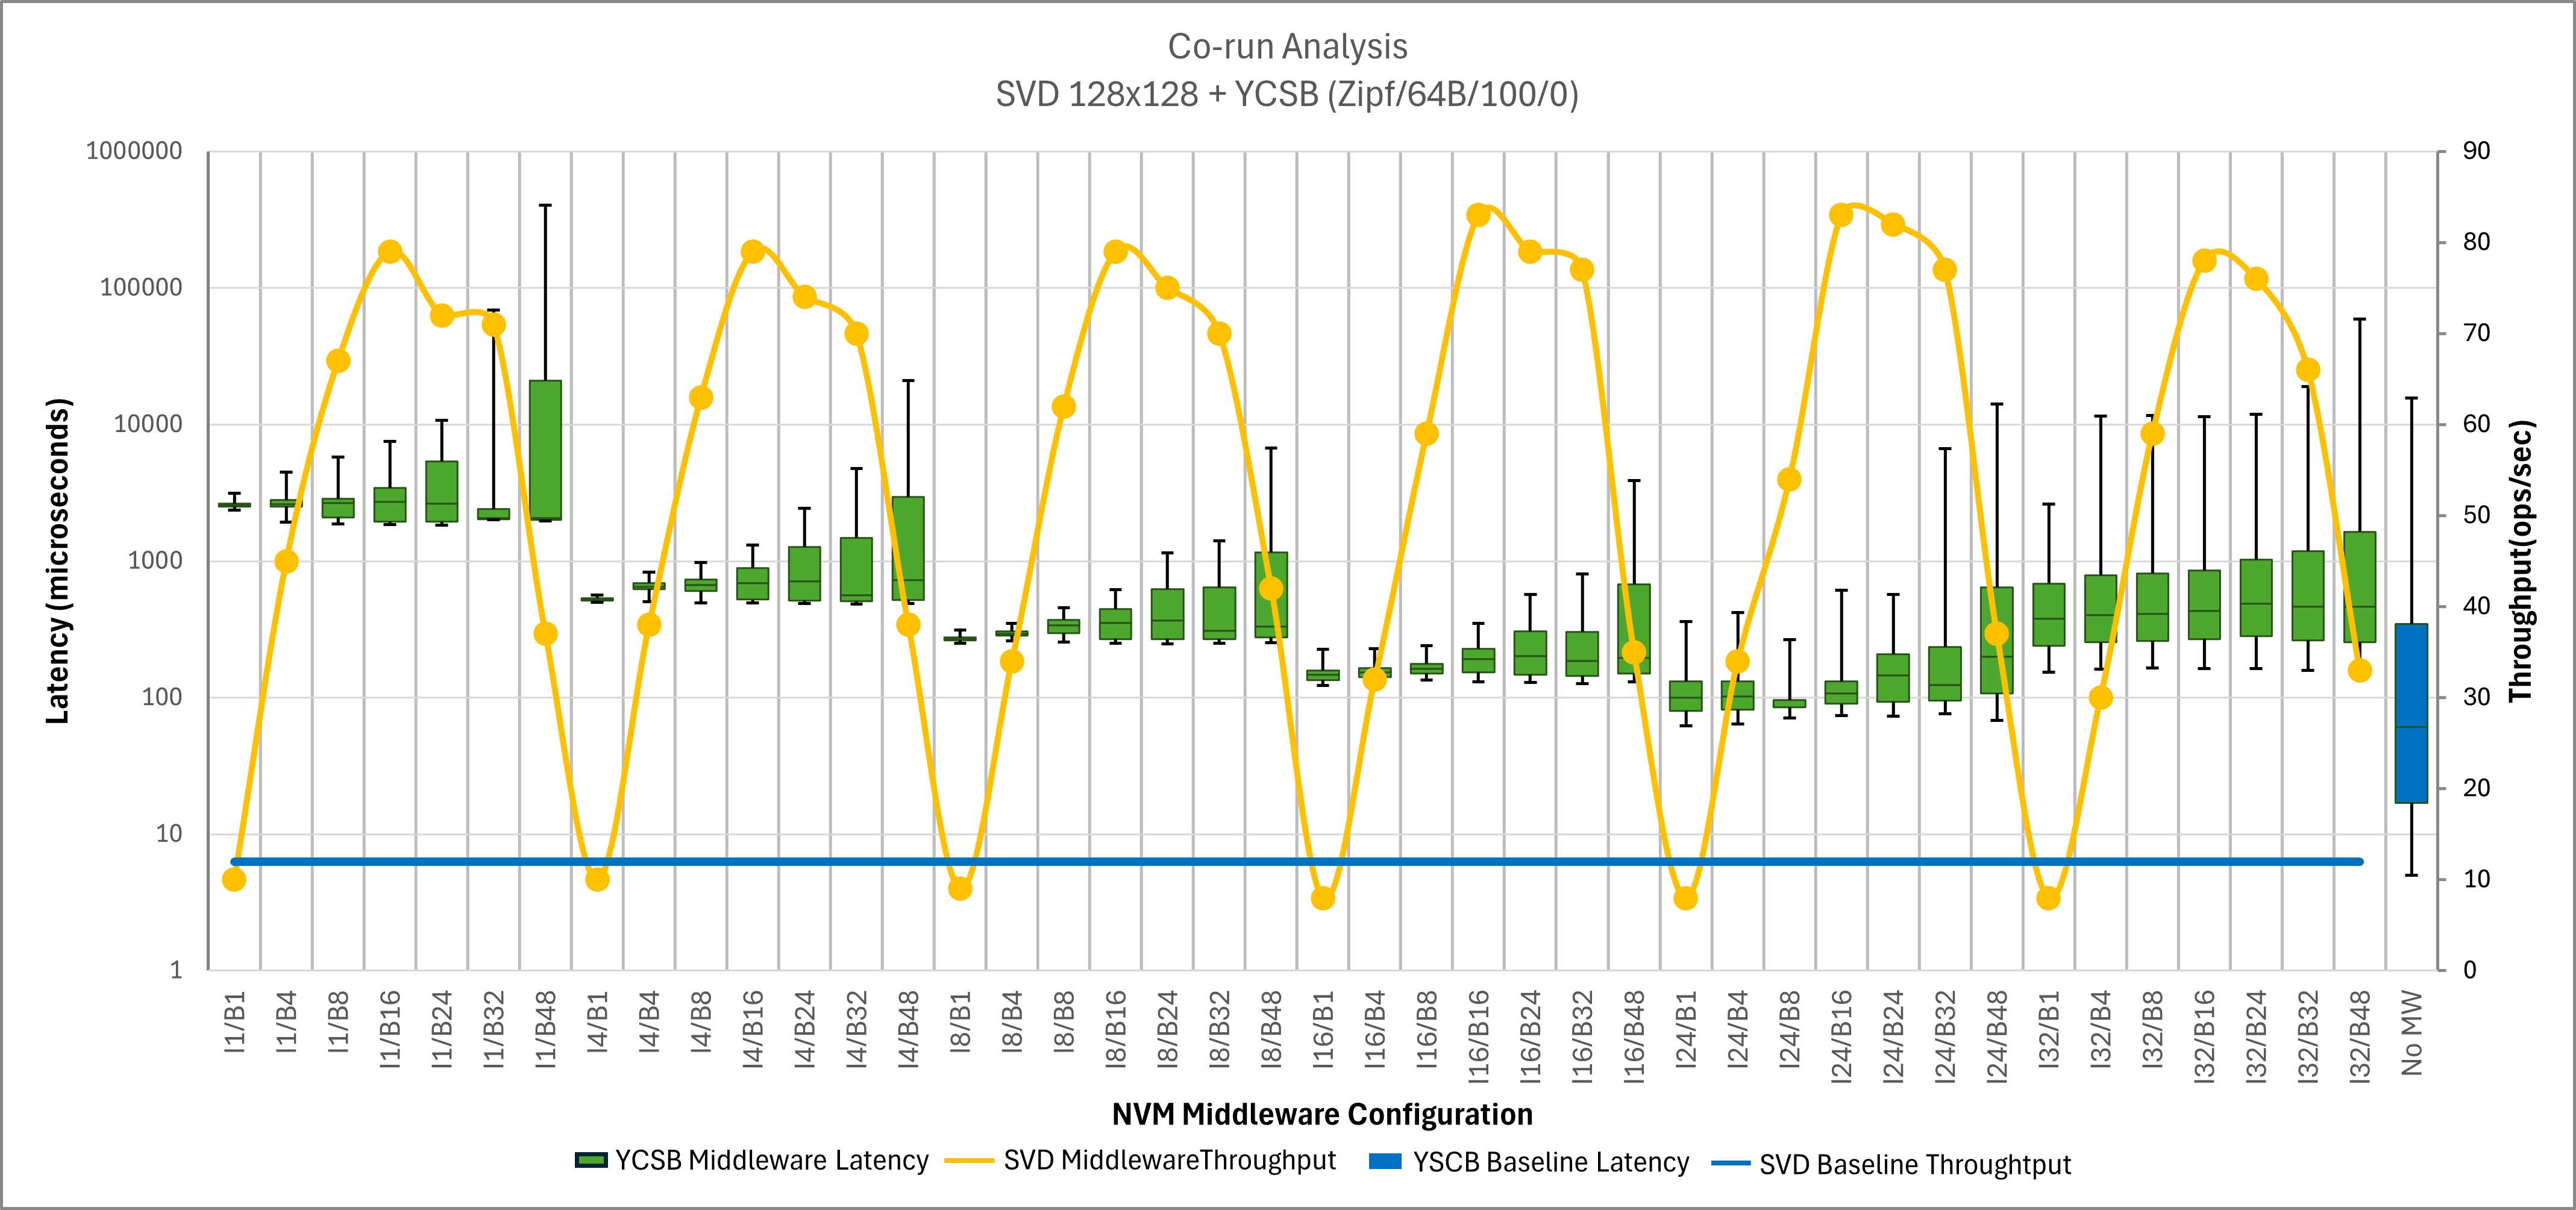
\includegraphics[width=0.8\textwidth,height=\textheight,keepaspectratio,angle=0]{images/64b_100_0_middleware_eval.png}
  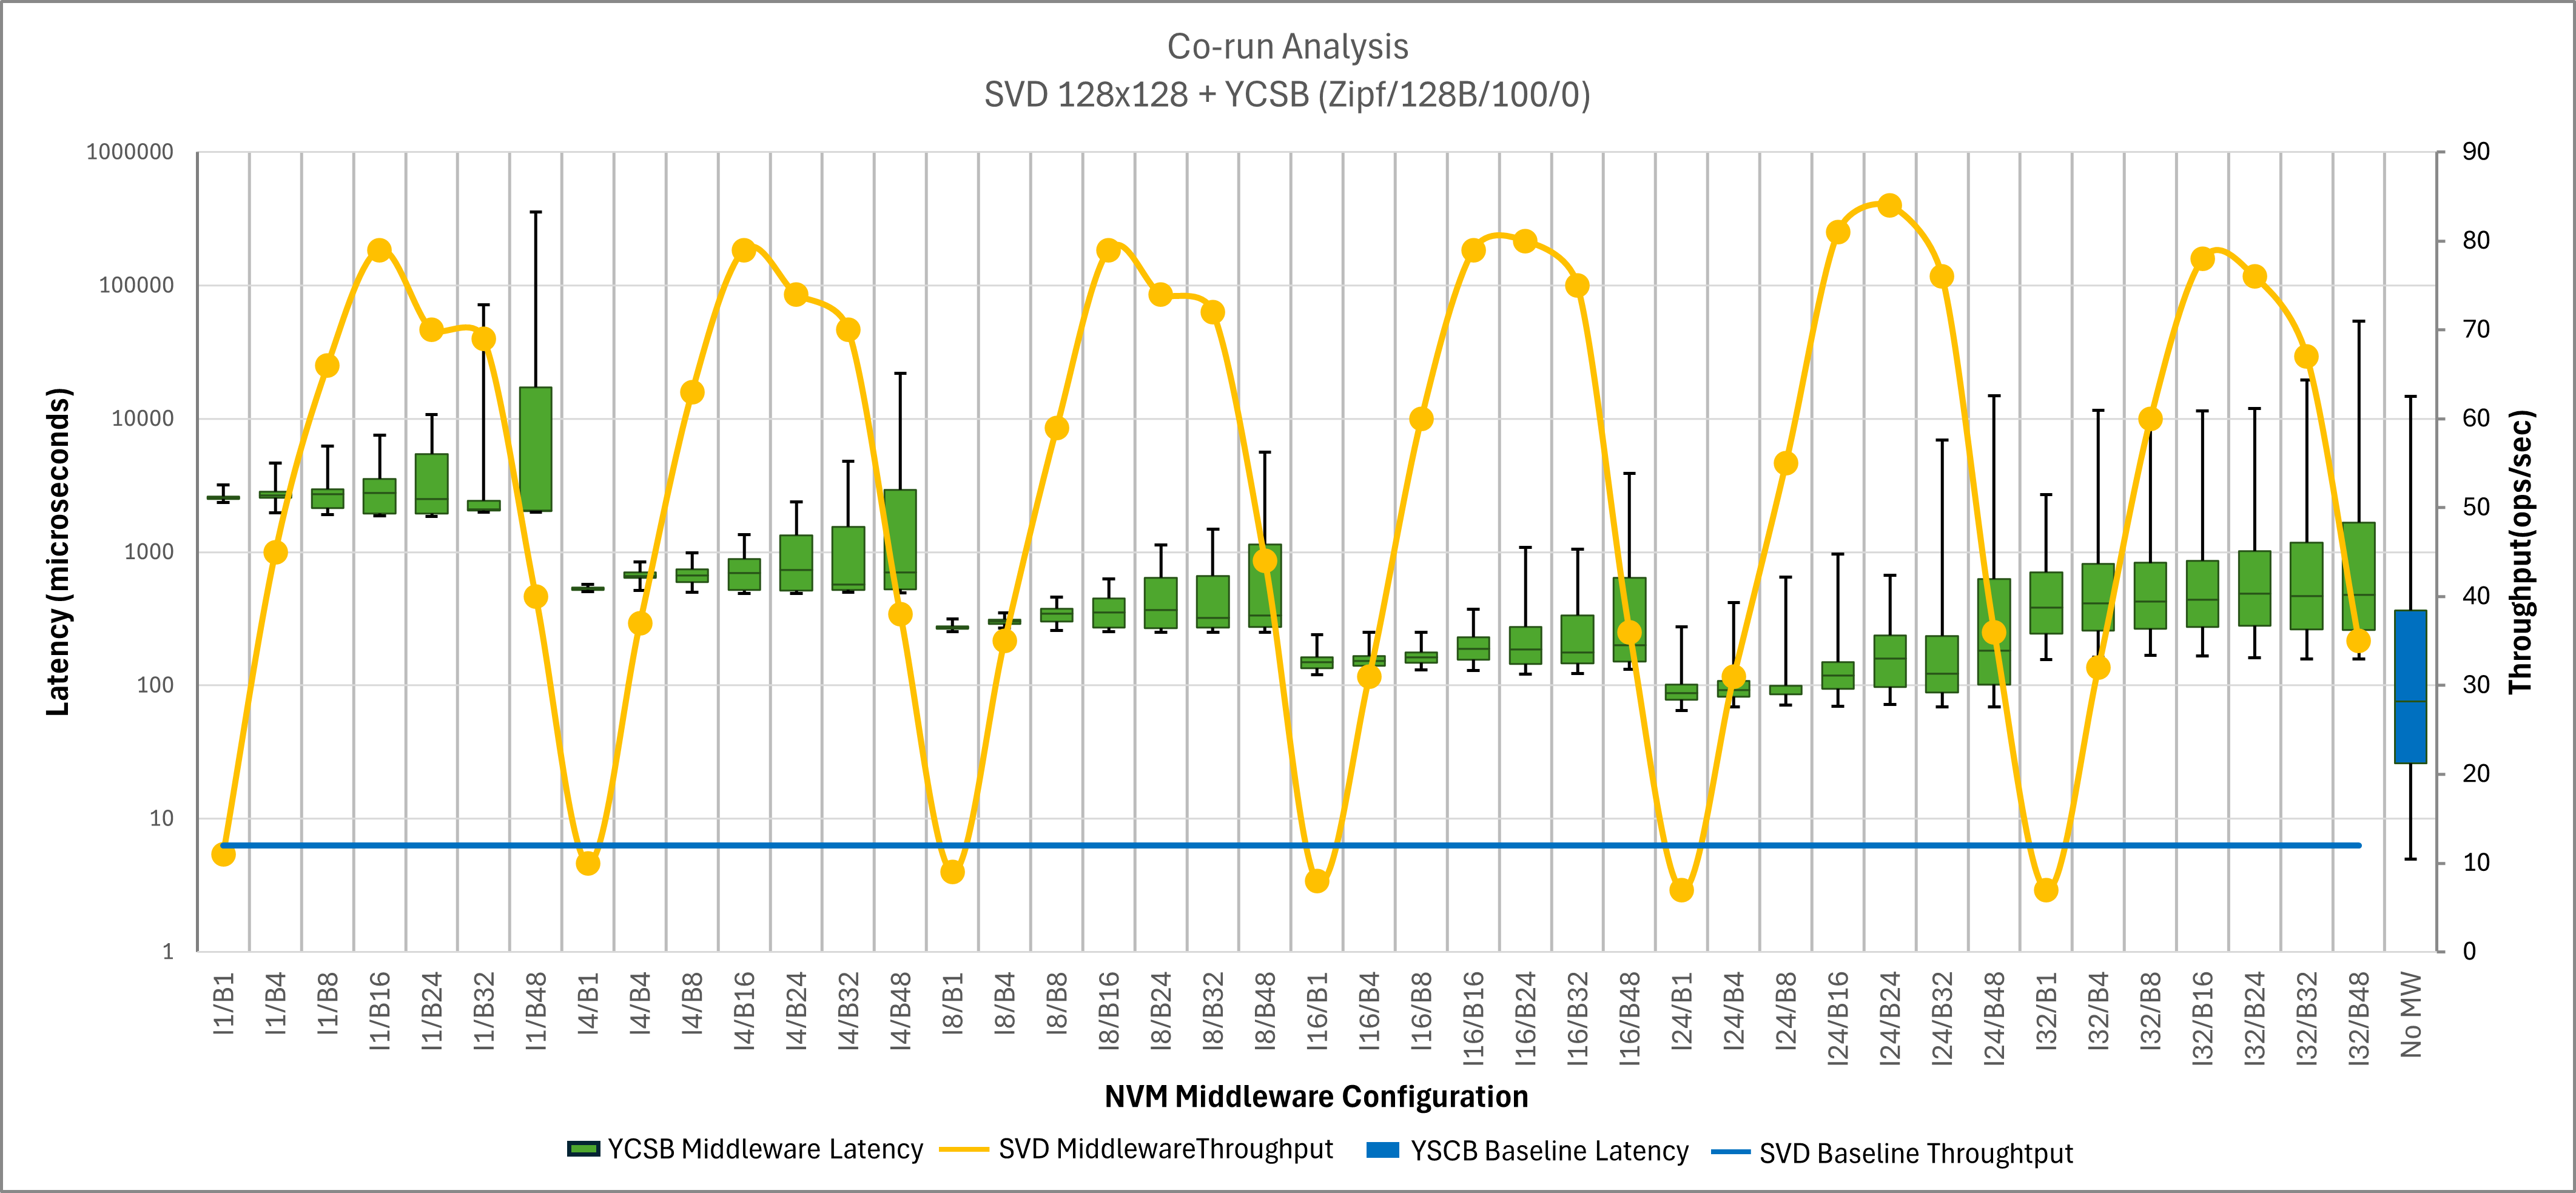
\includegraphics[width=0.8\textwidth,height=\textheight,keepaspectratio,angle=0]{images/128b_100_0_middleware_eval.png}
  % \caption[Evaluation of NVM Middleware: Benchmark B]{Evaluation of the NVM Middleware's concurrency control mechanism when co-running a batch workload and a pure read interactive workload with zipfian request distribution. The interactive workload is generated by YCSB, and two runs are performed configuring YCSB with 64B and 128B data access sizes. Both applications utilize 100 client threads to send requests to the NVM Middleware. The throughput (yellow line) and 99th percentile latency (green box plot) of each application are observed and compared against a baseline with no concurrency control (blue line and box plot).}
  \caption[Evaluation of NVM Middleware: Benchmark B]{Evaluation of the NVM Middleware's concurrency control mechanism when co-running SVD I/O traces and a pure read YCSB workload with Zipfian request distribution. Two runs are performed configuring YCSB with 64B and 128B data access sizes. Both applications utilize 100 client threads to send requests to the NVM Middleware.  The illustration presents statistics on throughput (yellow line) and 99th percentile latency (green box plot) obtained under different configurations of the NVM Middleware, denoted as $I/B$ (Interactive threads/Batch threads). These statistics are compared against a baseline scenario with no concurrency control (blue line and blue box plot). The latencies observed by YCSB are depicted as a distribution, ranging from the minimum to the maximum observed, along with quartiles and median values.}
  \label{fig:100_0_middleware_eval}
\end{figure}

\begin{figure}[ht]
  \centering
  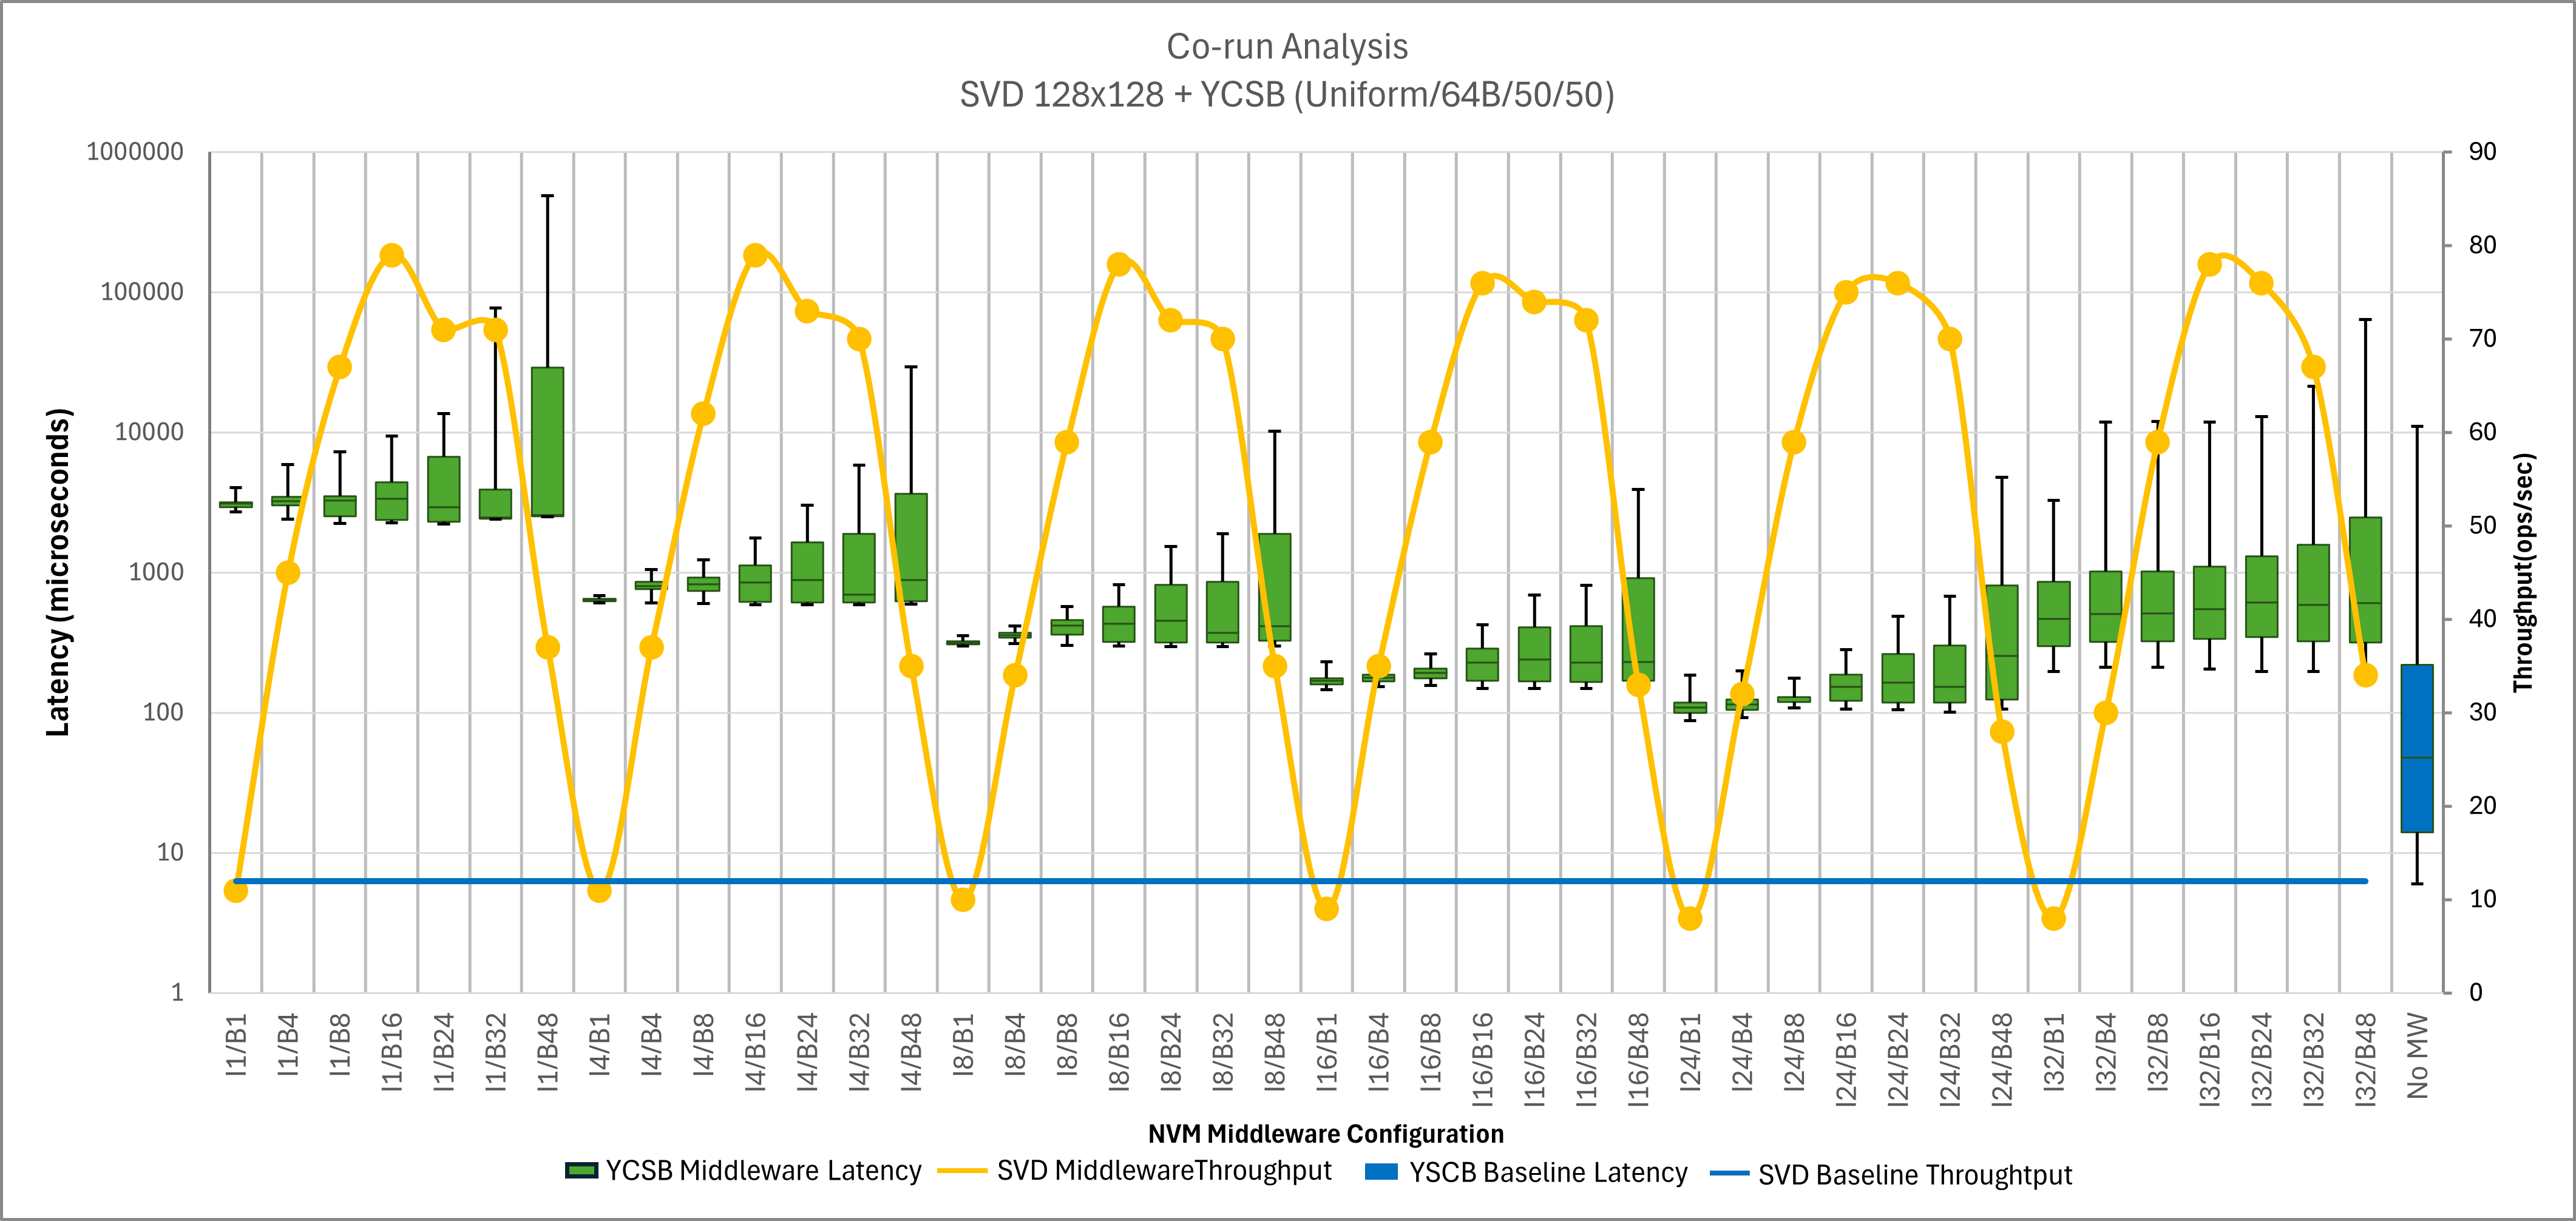
\includegraphics[width=0.8\textwidth,height=\textheight,keepaspectratio,angle=0]{images/64b_uniform_50_50_middleware_eval.png}
  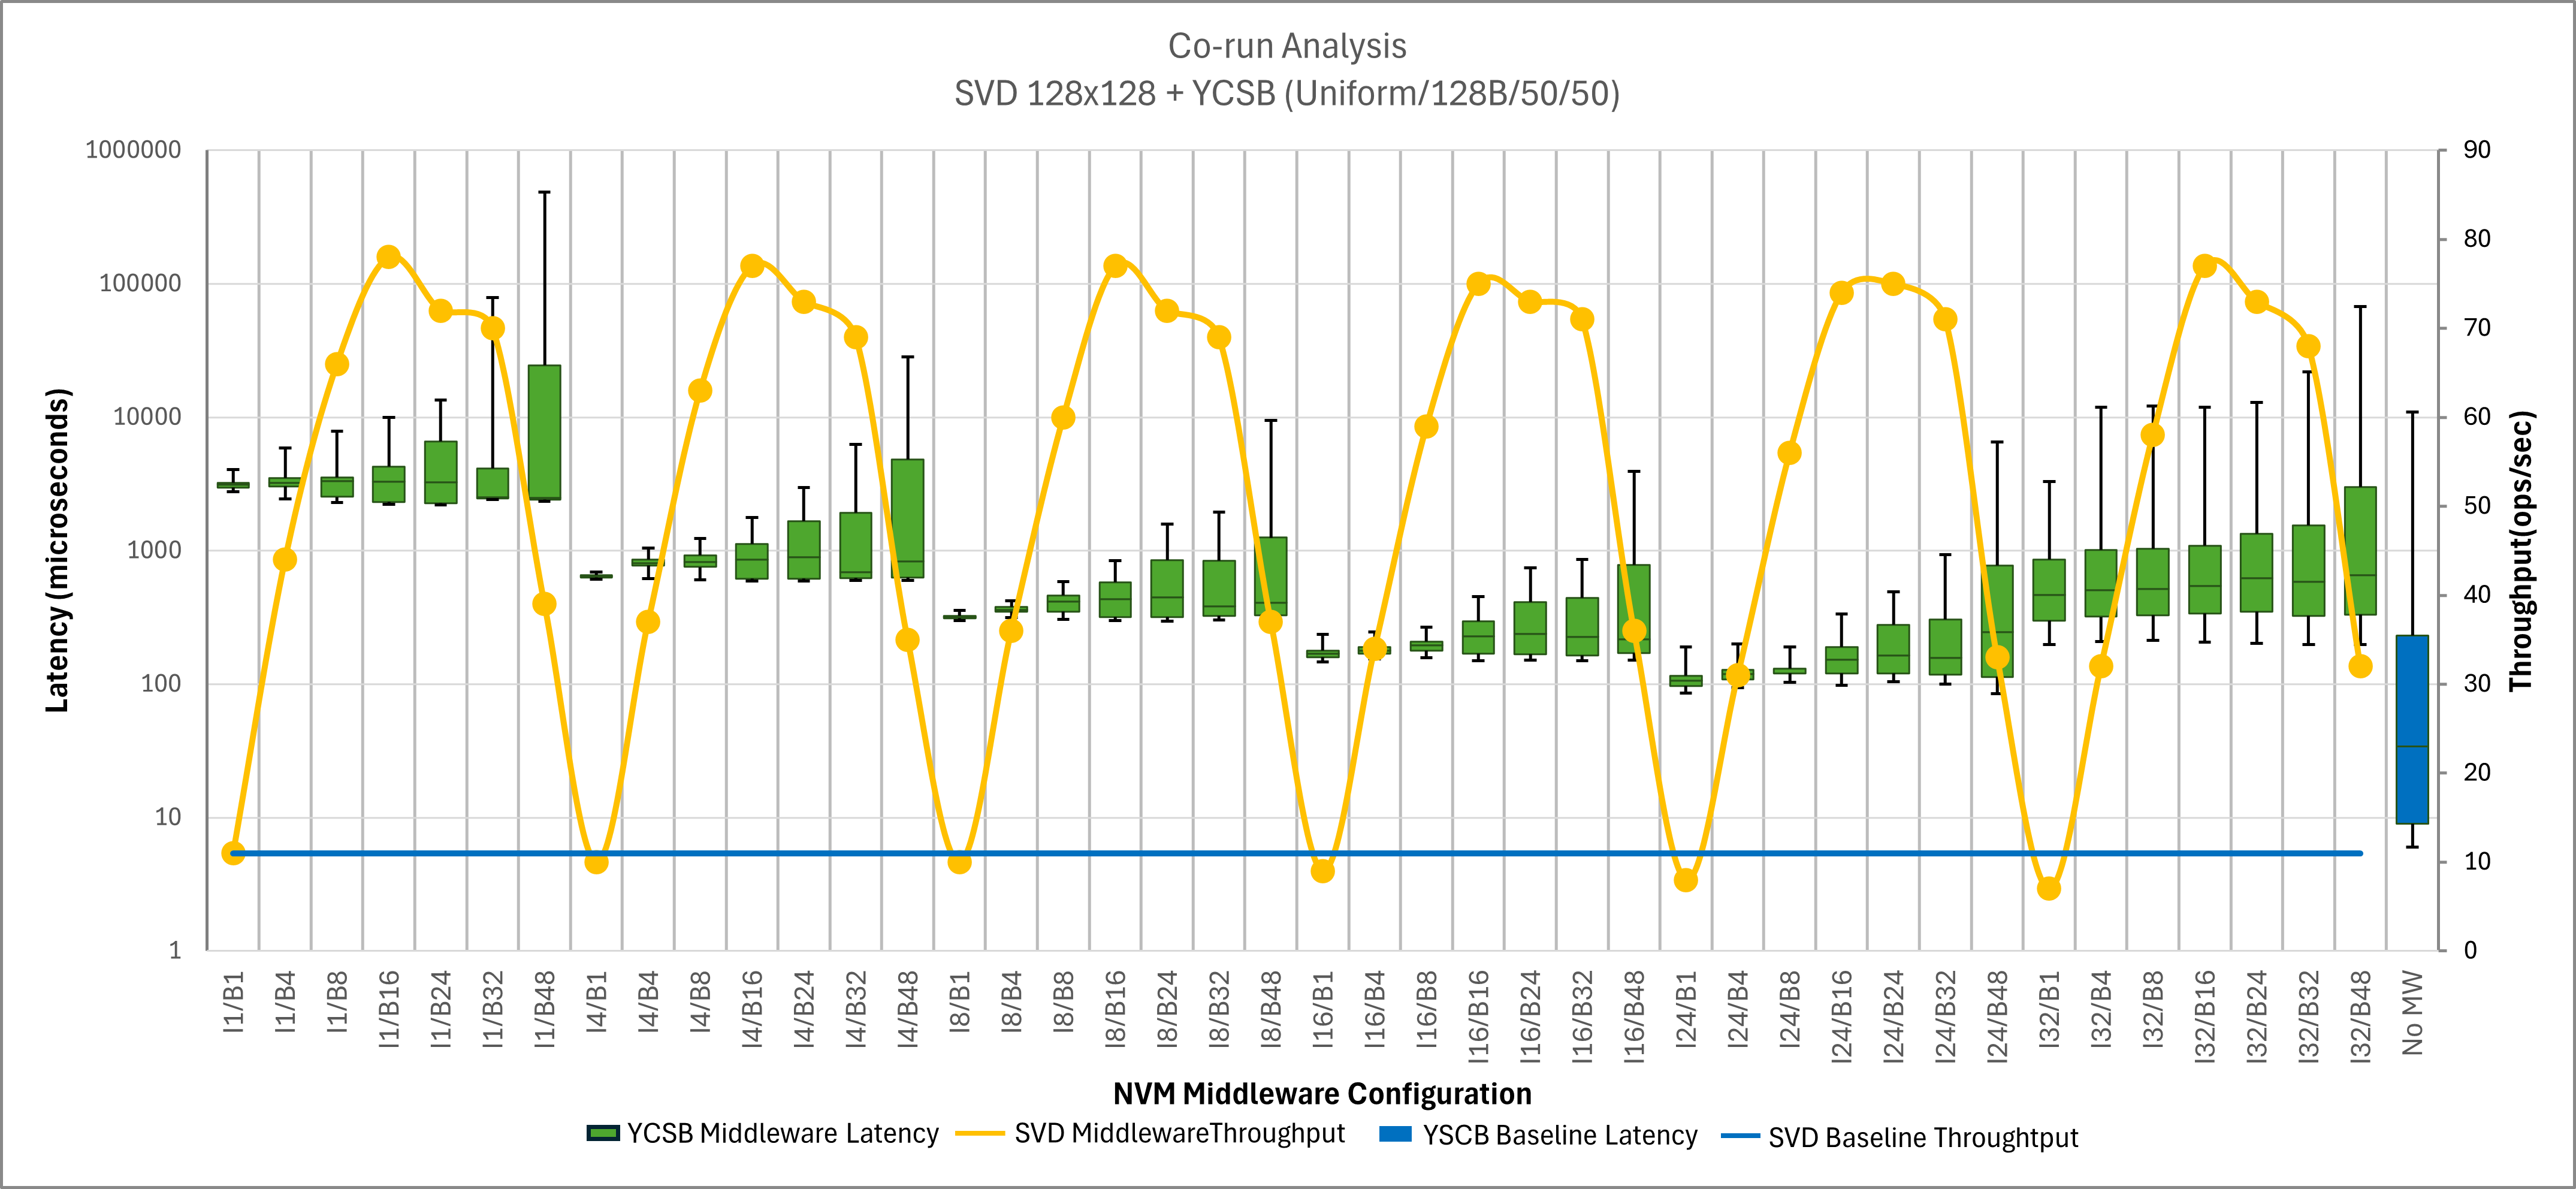
\includegraphics[width=0.8\textwidth,height=\textheight,keepaspectratio,angle=0]{images/128b_uniform_50_50_middleware_eval.png}
  % \caption{Evaluation C}
  % \caption[Evaluation of NVM Middleware: Benchmark C]{Evaluation of the NVM Middleware's concurrency control mechanism when co-running a batch workload and a YCSB workload configured with uniform request distribution and even distribution of read and write requests. The interactive workload is generated by YCSB, and two runs are performed configuring YCSB with 64B and 128B data access sizes. Both applications utilize 100 client threads to send requests to the NVM Middleware. The throughput (yellow line) of the SVD application and 99th percentile latency (green box plot) of YCSB are observed and compared against a baseline with no concurrency control (blue line and box plot).}
  \caption[Evaluation of NVM Middleware: Benchmark C]{Evaluation of the NVM Middleware's concurrency control mechanism when co-running SVD I/O traces and a YCSB workload configured with uniform request distribution and an even distribution of read and write requests. Two runs are performed configuring YCSB with 64B and 128B data access sizes. Both applications utilize 100 client threads to send requests to the NVM Middleware.  The illustration presents statistics on throughput (yellow line) and 99th percentile latency (green box plot) obtained under different configurations of the NVM Middleware, denoted as $I/B$ (Interactive threads/Batch threads). These statistics are compared against a baseline scenario with no concurrency control (blue line and blue box plot). The latencies observed by YCSB are depicted as a distribution, ranging from the minimum to the maximum observed, along with quartiles and median values.}
  \label{fig:uniform_50_50_middleware_eval}
\end{figure}